\chapter{Likelihood Point Estimation}
\label{chap:likelihood_point_estimation}
\minitoc
\section{Introduction}
Diffusion maps in \cref{chap:diff_maps} provide a good initial point estimate for fitting GIRG node locations to a real graph. However what we'd truly like to maximise is the actual data likelihood $p(G | \theta)$, where $G$ is the real graph and $\theta$ are all the GIRG parameters like $c, \alpha$, node weights and node locations. This is infeasible to compute exactly, but there have been many approximate methods developed in the literature for fitting HRGs. To our knowledge this is the first time that a point fitting attempt has been done for higher ($d=1,2,3$) dimensional GIRGs.

% In particular in \cref{sec:direct_ordered_likelihood_maximisation} we draw on ideas from \cite{garcia2019mercator}, and \cref{sec:mcmc_formulation} post-hoc has similarity to \cite{boguna2010sustaining}.


% we can use the likelihood to do a further refinement of point locations, although finding anything like a global optimum is infeasible for all but tiny graphs.

In \cref{sec:mcmc_formulation} we first tried a \textit{Markov Chain Monte Carlo (MCMC)} approach to not just improve $p(G | \theta)$, but also provide in theory an estimate of the posterior distribution of $p(\theta | G)$. Our use of the \textit{Metropolis-Hastings algorithm} turns out post-hoc to be similar (but less well implemented and analysed) to \cite{boguna2010sustaining}'s HRG fitting algorithm. We later shifted in \cref{sec:direct_ordered_likelihood_maximisation} to a \textit{direct ordered likelihood optimisation} with rounds of point location updates in order from highest to lowest degree node, inspired by \cite{garcia2019mercator}.


Though our methods are sadly not extremely well thought out or optimal, we still get reasonable results suggesting a good level of fit of the GIRG model already in just 1 dimension to the Facebook social networks, and evidence that adding more dimensions does not improve the fit much more.

\section{MCMC Formulation}
\label{sec:mcmc_formulation}
MCMC is a method in the bayesian framework of a parametric generative model. Datapoints $z$ are generated by first sampling $\theta \sim p(\theta)$ from a prior, and then generating from the model $z \sim p(z | \theta)$. In our case of fitting the GIRG GGM, $z$ is a real graph instance $G$, parameter $\theta = (\alpha, c, (w_u)_{u \in V}, (x_u)_{u \in V})$, and we focus in particular on the node locations $(x_u)_{u \in V}$.

The posterior likelihood $p(\theta | z) = \frac{p(z | \theta) p(\theta)}{p(z)}$ is infeasible to compute due to the normalising factor $p(z)$. MCMC instead uses the non-normalised $Q(\theta) = p(z | \theta) p(\theta)$ which can be evaluated, to set up a \textit{Markov Chain (MC)} with states $\theta \in \Theta$, and transition probabilities derived from $Q(\theta)$.
In particular we will use a \textbf{Metropolis-Hastings} style MC. The two basic components are a \textit{proposal distribution} to propse a new MC state $\theta' \sim p_{\mathrm{prop}}(\theta' | \theta)$, and an \textit{acceptance probability} $p_{\mathrm{acc}}(\theta' | \theta)$ to decide whether to accept $\theta'$. It might take a few rounds of proposal and rejection to produce one actual MC state transition. This defines  a random walk on the MC state space that converges in the limit to the posterior distribution $\theta \sim p(\theta | z)$. If the jth step of the random walk yields $\theta^j$, given sufficient burn in and spacing, we can sample $\theta^{j_1}, \theta^{j_2}, ...$ from the posterior. We will be content with just one posterior sampled $\hat{\theta}$ (NB not a maximum likelihood estimator), and use this to evaluate our overall GIRG model fit to the real graph.

We transition $\theta \to \theta'$ with a \textit{Gibbs sampling} approach. This means breaking down $\theta$ into subcomponents $\theta_i$, randomly choosing one to propose a new state for, i.e. $\theta' = (\theta'_i, \theta_{j:j \neq i})$, and using the marginal $Q_i(\theta_i)$ instead of $Q(\theta)$ in order to compute the transition probabilities.
In our case $Q(\theta) = p(G | (\vec{x}_u)_{u \in V}) p((\vec{x}_u)_{u \in V})$, so we can ignore the uniform prior $p((\vec{x}_u)_{u \in V})$ as it's constant for all node locations. Then we have 
\begin{align}
  & Q(\theta) \propto \prod_{(u,v) \in {V \choose 2}} p_{uv} | w_u, w_v, x_u, x_v, \alpha, c, G
  \\
  \text{easily marginalised as} \quad & Q_u(\theta_u) = \prod_{v \neq u} p_{uv} | ...
\end{align}
% which is easily marginalised as $Q_u(\theta_u) = \prod_{v \neq u} p_{uv} | ...$.
% This lends well to Gibb's sampling - we need concentrate only on $Q_u(\theta_u) = \prod_{v \neq u} p(e(u,v) | ...)$.

% Key elements of the MCMC approach are 1. burn in time, and 2. proposal distribution. 

\textit{Burn in time} of the MC can be quite long. With the GIRG model, the natural initialisation for $\vec{x}_u$ would be to follow the prior $\vec{x}_u \sim U([0, 1]^d)$. By using a diffusion map embedding initialisation this can be greatly reduced.

\paragraph{The proposal distribution} should be designed to maximise chances of acceptance. It seemed reasonable to randomly propose one of a small local perturbation, or a random jump to anywhere in the cube
% , with some probability of either (we elected for 70\% small perturbation).
A random uniform jump is useful to try and find a completely new location for $\vec{x}_u$ that could still be nicely near to $u$'s neighbours and far from its non-neighbours - in fact another good proposal would be to randomly choose a neighbour $v \sim u$, and move $\vec{x}_u$ to a random offset of $\vec{x}_v$, although this would unfortunately make $p_{\mathrm{prop}}$ no longer symmetric.
A small perturbation $\vec{x}_u' = \vec{x}_u + \epsilon$ is also good as, assuming that $\vec{x}_u$ has high likelihood, quite likely a nearby location will have an even higher one.

\paragraph{Acceptance probability} as defined by the Metropolis-Hasting's algorithm is
\begin{align}
  p_{\mathrm{acc}}(\vec{x}_u' | \vec{x}_u) &= \min \left (1,\;\;  \frac{p_{\mathrm{prop}}(\vec{x}_u | \vec{x}_u') p(G | \vec{x}_u') p(\vec{x}_u')}{p_{\mathrm{prop}}(\vec{x}_u' | \vec{x}_u) p(G | \vec{x}_u) p(\vec{x}_u)}\right )
  \\
  &= \min \left (1,\;\;  \frac{p(G | \vec{x}_u')}{p(G | \vec{x}_u)} \right )
  \\
  & \text{as $p_{\mathrm{prop}}$ is symmetric and $p(\vec{x}_u) = 1\; \forall \vec{x}_u$}
\end{align}

\begin{comment}
\section{Bayes Factor likelihood comparisons}
\begin{enumerate}
    \item Using one MCMC posterior sample of $\{x_u\}_{u \in V}$ and maximum likelihood estimates $\hat{\alpha}, \hat{c}, \hat{w}_u$, we estimate the likelihood $p(\cG_{\GIRG} | G)$, and can perform a comaprison $p(\cG_{\GIRG-1d} | G)$ vs $p(\cG_{\GIRG}-2d | G)$ vs $p(\cG_{CL} | G)$ etc.
    \item Results show that $p(\cG_{\GIRG}-1d | G)$ is better than 2D, 3D GIRGs, but not as good as Chung-Lu
    \item Results show that simply introducing a failure rate of $0.5$ onto the GIRGs (unfortunately not correcting for LCC), the model probabiltiy estimate for 1D GIRG then beats out Chung-Lu (all copyweights)
\end{enumerate}


What the heck is Bayes Factor anyway?

Apparently it's basically comparing $P(M_1 | D)$ and $P(M_2 | D)$. In our case $M_1, M_2$ is e.g. 1D GIRG vs 2D GIRG, and $D$ the data is just one graph instance. We have some prior of $P(M_1)$ vs $P(M_2)$, e.g. 50-50, or some kind of decaying $1D \GIRG > 2D \GIRG > 3D \GIRG > \dots$.

Then the comparison is $P(M_1 | D) = \frac{P(D | M_1) P(M_1)}{P(D)}$. I.e. the ratio $\frac{P(M_1 | D)}{P(M_2 | D)}$ is the ratio $\frac{P(D | M_1) P(M_1)}{P(D | M_2) P(M_2)}$.

We will ignore the priors $P(M_1), P(M_2)$, for now, and focus on the likelihoods $P(D | M_1), P(D | M_2)$. In our case if $M_1$ is a 1D GIRG, and we've decided to fix e.g. $\alpha, e, \{w_u\}_{u \in V}$, and just vary $\theta = c, \{x_u\}_{u \in V}$, then we could monte-carlo sample $\theta \sim p(\theta)$ from the prior to get an estimate, $P(D | M_1) = P(G) = \int_\theta P(G | \theta) p(\theta) d\theta$, where we drop the $| M_1$ as we've fix into the 1D GIRG universe.

This seems inefficient. Instead we can sample $\theta \sim P(\theta | G)$ from the posterior using MCMC, and then evaluate  

\begin{align*}
    1/P(G) 
        &= \int_\theta \frac{1}{P(G)} P(\theta) d\theta
        \\
        &= \int_\theta \frac{P(\theta, G)}{P(G)} \frac{1}{P(\theta, G)} P(\theta) d\theta 
        \\
        &= \int_\theta P(\theta | G) \frac{P(\theta)}{P(\theta, G)} d \theta
        \\
        &= \int_\theta P(\theta | G) \frac{1}{P(G | \theta)} d\theta
        \\
        &= E_{\theta \sim \theta | G} \left [ \frac{1}{P(G | \theta)} \right ]
        % &= \int_\theta P(\theta) P(G | \theta) d\theta
        % \\
        % &= \int_\theta P(\theta) \frac{P(\theta | G)}{P(\theta | G)} P(G | \theta) d\theta
        % \\
        % &= \int_\theta \frac{P(G, \theta)}{P(\theta | G)} P(\theta | G) d\theta
        % \\
        % &= \int_\theta \frac{P(G | \tehta) | \theta}
\end{align*}

The good news is that while MCMC sampling from $P(\theta | G)$, it seems that the likelihood $P(G | \theta)$ is relatively consistent.

TODO think through more penalisation of models by parameter count. Does this $P(G)$ calculation take this into account already? I.e. a high parameter count model can fit many different $G$, so although $G$ is more \q{plausible} under a higher count model, there are also more alternative outcomes $G'$ so as to dilute the probability?
\end{comment}

\subsection{MCMC likelihood comparison of GIRG vs CL fit to real graph}
How well do the converged MCMC points do at replicating the real graph? As suggested in the classification comparison framework, the Chung-Lu model is a good non-geometric null hypothesis to compare against - i.e. we hope that the MCMC fit GIRG model will do better than Chung-Lu. It's also interesting to see how large a dimension $d$ is necessary for a good GIRG fit.

As a first sanity check, we compare the MCMC fit $\hat{\theta}_{\GIRG}$ to the more simply fit copy-weight Chung-Lu parameters $\hat{\theta}_{CL}$, by comparing $p(G | \hat{\theta}_{\GIRG}, \cG_{\GIRG})$ vs $p(G | \hat{\theta}_{CL}, \cG_{CL})$. 

For most of the facebook graphs however, $p(G | \hat{\theta}_{\GIRG}, \cG_{\GIRG}) < p(G | \hat{\theta}_{CL}, \cG_{CL})$, despite GIRGs having more parameters / flexibility to fit $G$!

The GIRG model is far too confident about edges, giving $p_{uv} \approxeq 1$ for small $\norm{x_u - x_v}$ and $p_{uv} \approxeq 0$ for large $\norm{x_u - x_v}$. Hence a mistake on a few edges can lead to a large penalisation in likelihood. The Chung-Lu model is much more forgiving, with all probabilities more medium sized. 

% by evaluating the likelihood $p(G | \hat{\theta}, \cG)$ for both models. We expect that the GIRG model will do better, as it has more parameters to fit, and is more flexible.
% we can sample a $\hat{\theta}_{\GIRG}$ (not MLE but still pretty good) as from the posterior $\theta_{\GIRG} | G$ with MCMC, and more simply fit a $\hat{\theta}_{CL}$. Given that the 1D GIRG is a more parametrised model, it would be total failure if it didn't reproduce the given graph better. For most of the facebook graphs however, $p(G | \hat{\theta}_{\GIRG}, \cG_{\GIRG}) < p(G | \hat{\theta}_{CL}, \cG_{CL})$!
% The GIRG model is far too confident about edges, giving $p_{uv} \approxeq 1$ for small $\norm{x_u - x_v}$ and $p_{uv} \approxeq 0$ for large $\norm{x_u - x_v}$. Hence a mistake on a few edges can lead to a large penalisation in likelihood. The Chung-Lu model is much more forgiving, with all probabilities more medium sized. 

One reasonable tweak is to introduce a \textit{failure rate} $0 \leq f \leq 1$ to the GIRG model: 
% $p_{uv} = (1-f) \min( ... )$
\begin{equation}
  p_{uv} = (1 - f) \min \left \{ 
    1,
    c \left (
        \frac{w_u w_v / W}{\norm{x_u - x_v}^d}
    \right )^\alpha    
\right \}
\end{equation}
For a social network this means that two highly similar people are not guaranteed/forced to be friends. Indeed there may be a very like-minded person who lives next door to you that you've never met, or had no opportunity / free time to properly get to know.

A failure rate will lower the impact of short non-edges (mistakenly predicted with a high edge probability), but for long edges (mistakenly predicted with a low edge probablity) we need a baseline edge probability to prevent $p_{uv}$ being too small. A simple fix is a \textit{mixture probability} of deriving edges instead from the Chung-Lu model - i.e. letting
\begin{equation}
  p_{uv} = \eta \; p_{uv}^{CL} + (1 - \eta) \; p_{uv}^{GIRG}
\end{equation}
for mixture probability $0 \leq \eta \leq 1$. This should not be seen strictly as an ensemble of models or gross addition to the number of parameters of the GIRG model, as the GIRG model already contains fit node weights $(\hat{w}_u)_{u \in V}$. The mixture probability $\eta$ does also help a lot on short non-edges similarly to failure rate $f$, but it could still be good to have both as even the Chung-Lu model can demand an edge $u \sim v$ with high probability if $w_u, w_v$ are both very large - though this is quite rare.

The intuitive social network interpretation of a GIRG Chung-Lu mixture model is that it allows for some \q{random} friendships - ones that wouldn't normally have been predicted by the GIRG model. For instance if you happen to sit next to a stranger on a plane, as long as they don't fall into a sworn enemy category you may still add them as a facebook friend with a vague promise of staying in touch. Of course you and the stranger must bear at least some small similarity to have been on the same plane, but this would likely need a very high dimensional GIRG model to be fully captured. 


With these two new parameters $f$ and $\eta$, the augmented GIRG model does have a higher specific fit likelihood than the Chung-Lu model: $p(G | \hat{\theta}_{GIRG}, \cG_{GIRG}) > p(G | \hat{\theta}_{CL}, \cG_{CL})$. In a holistic MCMC setup these two parameters could also have a prior and be sampled from the posterior, but for simplicity we set them to $f=0.3, \eta=0.5$, which perform reasonably. See \cref{fig:mcmc_runs} for some likelihood convergence curves on some example graphs. If we don't use a failure rate and mixture probability, the MCMC actually converges to a perverse set of node locations that are almost uniform, i.e. striving to be far apart, due to the high penalty cost of short non-edges.


% TODO Must input graphs here hold up


\begin{figure}
  \centering

  \begin{subfigure}{0.49\textwidth}
    \centering
    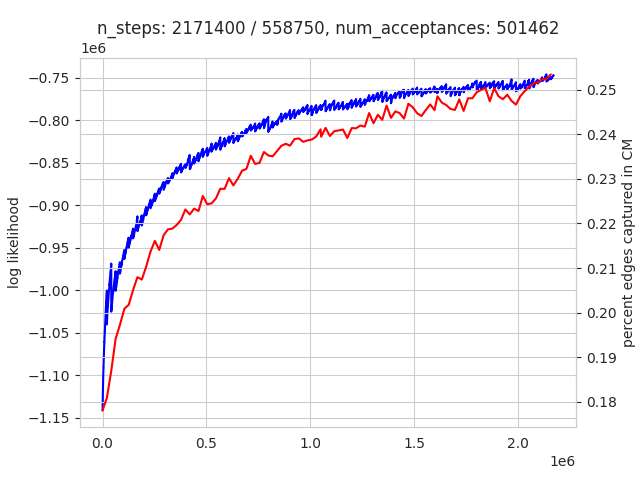
\includegraphics[width=\linewidth]{figures/MCMC_plots/socfb-Amherst41-1d.png}
    \caption{Amherst41 $d=1$}
  \end{subfigure}
  \hfill
  \begin{subfigure}{0.49\textwidth}
    \centering
    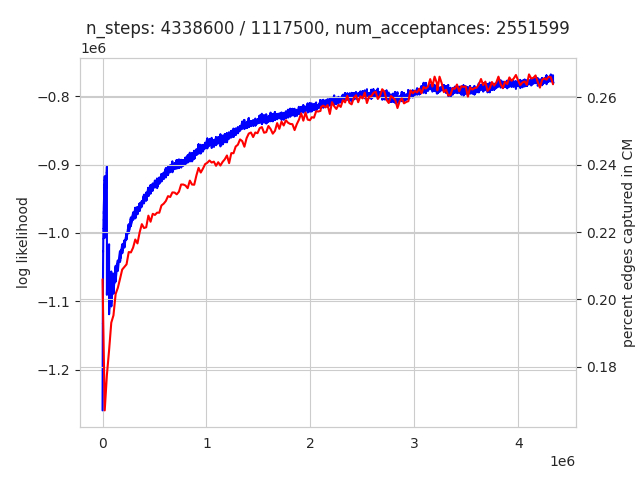
\includegraphics[width=\linewidth]{figures/MCMC_plots/socfb-Amherst41-2d.png}
    \caption{Amherst41 $d=2$}
  \end{subfigure}

  \vspace{1em}

  \begin{subfigure}{0.49\textwidth}
    \centering
    \includegraphics[width=\linewidth]{figures/MCMC_plots/socfb-Trinity100-1d.png}
    \caption{Trinity100 $d=1$}
  \end{subfigure}
  \hfill
  \begin{subfigure}{0.49\textwidth}
    \centering
    \includegraphics[width=\linewidth]{figures/MCMC_plots/socfb-Trinity100-2d.png}
    \caption{Trinity100 $d=2$}
  \end{subfigure}

  \vspace{1em}
  \begin{subfigure}{0.49\textwidth}
    \centering
    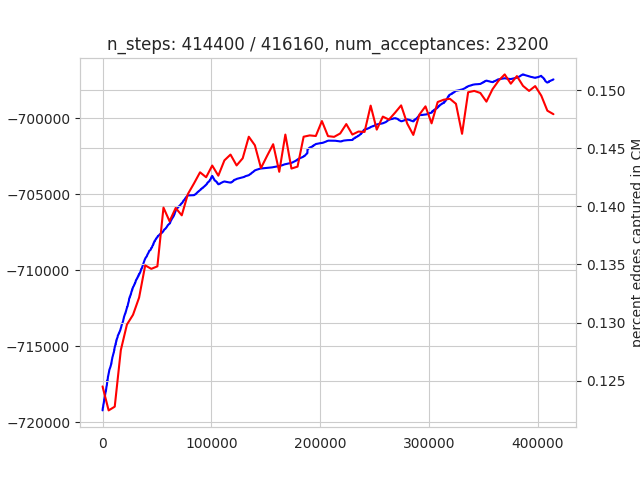
\includegraphics[width=\linewidth]{figures/MCMC_plots/socfb-Hamilton46-1d.png}
    \caption{Hamilton46 $d=1$}
  \end{subfigure}
  \hfill
  \begin{subfigure}{0.49\textwidth}
    \centering
    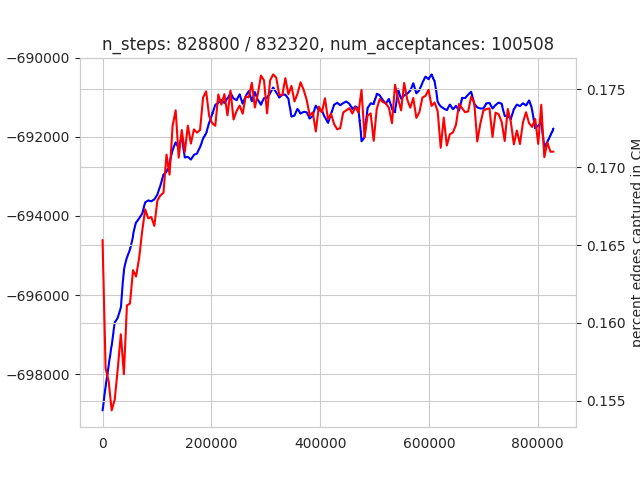
\includegraphics[width=\linewidth]{figures/MCMC_plots/socfb-Hamilton46-2d.png}
    \caption{Hamilton46 $d=2$}
  \end{subfigure}

  % \vspace{1em}
  % \begin{subfigure}{0.49\textwidth}
  %   \centering
  %   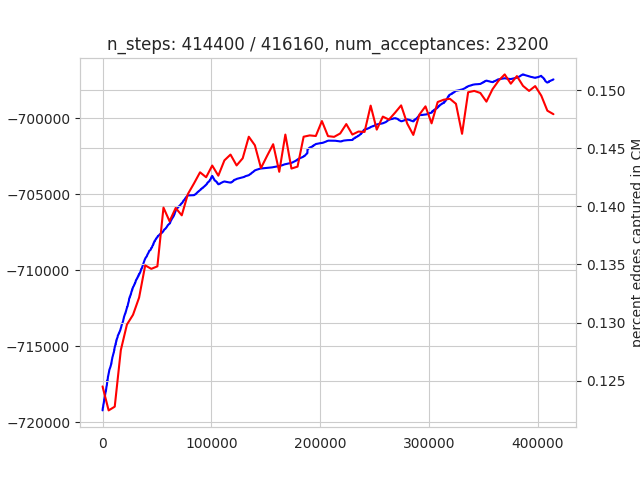
\includegraphics[width=\linewidth]{figures/MCMC_plots/socfb-Hamilton46-1d.png}
  %   \caption{$d=1$}
  % \end{subfigure}
  % \hfill
  % \begin{subfigure}{0.49\textwidth}
  %   \centering
  %   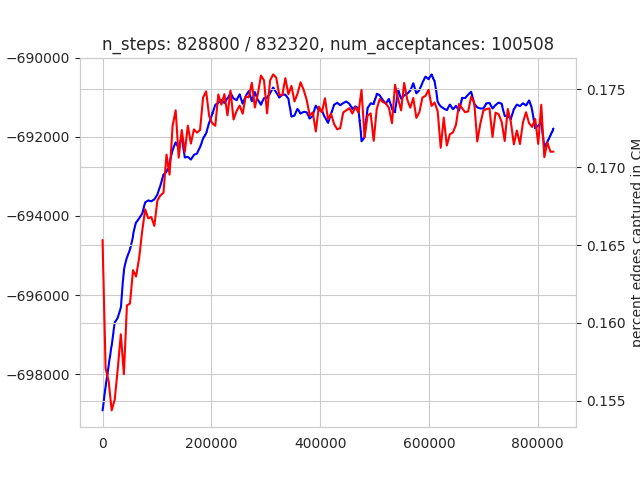
\includegraphics[width=\linewidth]{figures/MCMC_plots/socfb-Hamilton46-2d.png}
  %   \caption{$d=2$}
  % \end{subfigure}

  % \vspace{1em}
  % \begin{subfigure}{0.49\textwidth}
  %   \centering
  %   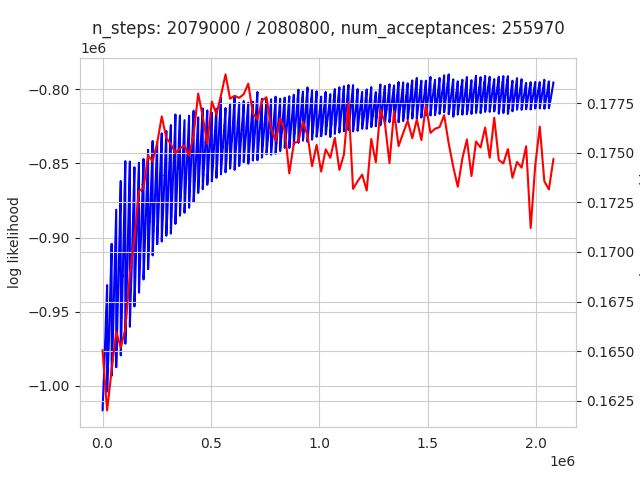
\includegraphics[width=\linewidth]{figures/MCMC_plots/socfb-Hamilton46-3d.png}
  %   \caption{$d=1$}
  % \end{subfigure}
  % \hfill
  % \begin{subfigure}{0.49\textwidth}
  %   \centering
  %   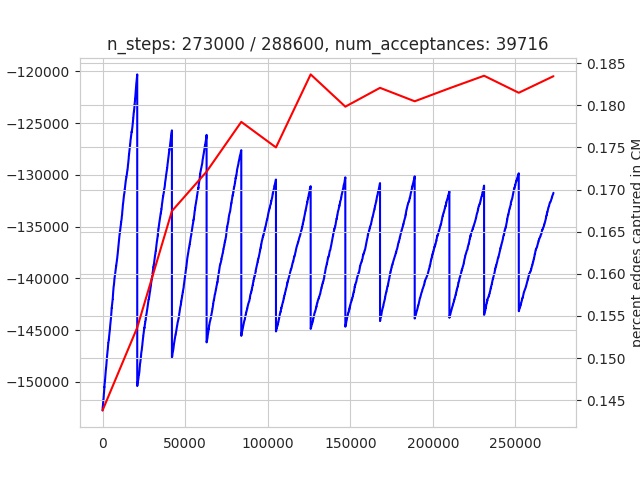
\includegraphics[width=\linewidth]{figures/MCMC_plots/socfb-Reed98-1d.png}
  %   \caption{$d=2$}
  % \end{subfigure}

  % \vspace{1em}


  \caption{MCMC runs for socfb-Amherst41, sofcb-Trinity100, socfb-Hamilton46 with failure rate $0.3$ and Chung-Lu Mixin rate $0.5$, with a cube GIRG model. Log likelihood wise, Amherst 1D GIRG does best; for Bowdoin it's 2D GIRG.
  x-axis is number of steps; left y-axis (blue curve) is log likelihood; right y-axis (red curve) is PEC metric}
  \label{fig:mcmc_runs}
\end{figure}

\subsection{Percent Edges Captured Metric Comparison}
A good and simple framework to compare quality of fit without taking into account increased parametrisation is to analyse the \q{accuracy} on successfully producing edges / non-edges.

Our MCMC posterior is constrained by directly fitting $\hat{c}$ to produce a similar number of edges $|E|$ as in the real graph. Hence in the standard classification confusion matrix
\begin{equation}
  \begin{array}{|c|c|}
    \hline
    TP & FN \\
    \hline
    FP & TN \\
    \hline
    \end{array}
\end{equation}
we can equivalently count $\frac{TP}{TP + FN}$ (Recall), the fraction of edges in the real graph that are successfully predicted, or $\frac{TP}{TP + FP}$ (Precision), the fraction of edges in the predicted graph that are also in the real graph, these numbers will be very similar. We call this metric \textit{Percent Edges Captured (PEC)}, and focus on this instead of the alternative Percent Non-Edges Captured (PNEC). PEC is preferrable as our graphs are all relatively sparse - hence the PNEC is always high as it is dominated by the large number of non-edges.


\section{Direct Ordered Likelihood Maximisation}
\label{sec:direct_ordered_likelihood_maximisation}
MCMC proved too slow and didn't achieve such high PECs. Hence we shifted to a slightly faster and simpler approach inspired by \cite{garcia2019mercator}'s  \textit{Mercator} monikered method.

Instead of picking points to update randomly, we sequentially update the positions of every single node, ordered from highest to lowest degree; Mercator uses a more sophisticated ordering based on the \textit{onion-decomposition} of the input graph. Updating point $\vec{x}_u$ is done by proposing $100$ new locations (Mercator actually suggests $O(\log n)$) near to current location, near to a neighbour, or random uniform in the cube. Instead of using an acceptance probability as in MCMC, we simply pick the best of all the proposals, by marginal edge likelihood $\prod_{v \neq u} p(e(u,v) | ...)$.

Updating points in order of highest degree makes sense as in essence a high degree node \q{drags} its local lower degree neighbourhood of nodes along with it, and thus should be updated in that order - otherwise if its lower degree neighbours are moved first, they might spread out more nonsensically and leave the higher degree node no good place to move to. We think this happened to some extent with the MCMC method, evidenced by initial drops in the PEC in \cref{fig:mcmc_runs} for 2d GIRG fits.

After each round of point updates, $\alpha$ is fit to maximise the likelihood, and $c$ is refit to match the number of edges in the real graph, similarly as in \cref{subsec:fitting_c_and_alpha}. Multiple rounds are repeated until convergence. One optimisation that Mercator implements but we missed was to also after each round update node weight estimates: comparing two nodes with similar degree, if the first one has more geometrically close nodes than the second, the second should have a relatively higher estimated weight.



\subsection{Ideas for speeding up convergence}
TODO Finish writing this section!!!

In fact the Mercator method doesn't do rounds of point updates, they are confident in node locations after just one round. \cite{boguna2010sustaining} similarly seeks to minimise computation by only doing iterative Metropolis-Hastings updates on higher degree nodes - fitting locations for lower degree nodes just once. Both papers deal with fittig HRGs; unfortunately higher dimensioned GIRGs have even more issues with speed of fitting locations due to an expanded search space. We present some ideas for speeding up convergence in a related vein that could be explored more in future work.

\paragraph{Gradient based point proposals}
When randomly proposing $100$ (or $O(\log n)$) new locations for each node, the resultant likelihood contribution of each location has to be computed. The number of locations would likely need to be exponentially increased for larger dimensions $d$ to achieve convergence.
An cheaper alternative is to just have one good proposal which is not random, rather taken as a small step in the direction of the gradient of the node likelihood contribution with respect to its location.
% We can speed this up by instead calculating the point location gradient of the likelihood contribution of each node, and taking a small step in the proposed direction.
We did limited tests which indeed showed faster convergence, but in general to a lower PEC value than before. One issue seemed that a much lower learning rate (step length in gradient direction) might be needed for $d=1$ compared to higher dimensions: for $d=1$, a node has neighbours and non-neighbours to the left and right, and will end up with quite a strong gradient pointing in one of the two directions, whereas for $d \geq 2$ forces on the node are in all different directions and hence more likely to be more finely balanced out with a smaller resultant gradient. Gradient clipping could potentially help.
Another issues is that without random new point location proposals, nodes could easily get stuck in local optima.

\paragraph{Sequential dimension fitting}
For real graphs, there is generally a steeper decrease in marginal benefit from adding dimensions than from strictly GIRG generated graphs. Hence a point fitting approach that is sequential in dimensions could make sense. We could first fit the first (and hence picked up as most important dimension) of every node. Then holding this fixed, fit the second dimension of every node, and so on. In essence it switches an exponential in $d$ search space scaling to be just linear in $d$. This is similar to an iterative eigenvalue algorithm.

This sequential dimension fitting would of course have similar local optima issues. A simple example is a $d=2$ MCD GIRG setting with three nodes $A,B,C$, where $A \sim B;\; B \sim C;\; A \nsim C$. Fitting the first dimension, the nodes would be placed in a line as A-B-C, to try and maximise the A-C distance while minimising A-B, B-C. This would unfortunately still lead A-C to be not so small due to the triangle inequality, which could not be improved when fitting the second dimension. The true optimal solution would be to have A-B close in the first dimension, B-C close in the second dimension, and A-C far in both dimensions.


\subsection{Analysis of quality of fit of GIRGs to real graphs}
We see in \cref{fig:converged_pecs} the final achieved PECs of different dimensional cube GIRGs fit to real-world graphs. At first blush, PECs seem worryingly low at just $22\%$ to $32\%$. You wouldn't be happy with a cat image classifier with only $30\%$ accuracy!
Furthermore, PEC decreases with increasing node count which seems to imply that our model fitting could be a fluke that only works on smaller graphs, and that might scale to irrelevance for even larger graphs.
Luckily all these signs of disaster have good explanations, and we can mostly restore faith in our point fitting methods.

\begin{figure}
  \centering
  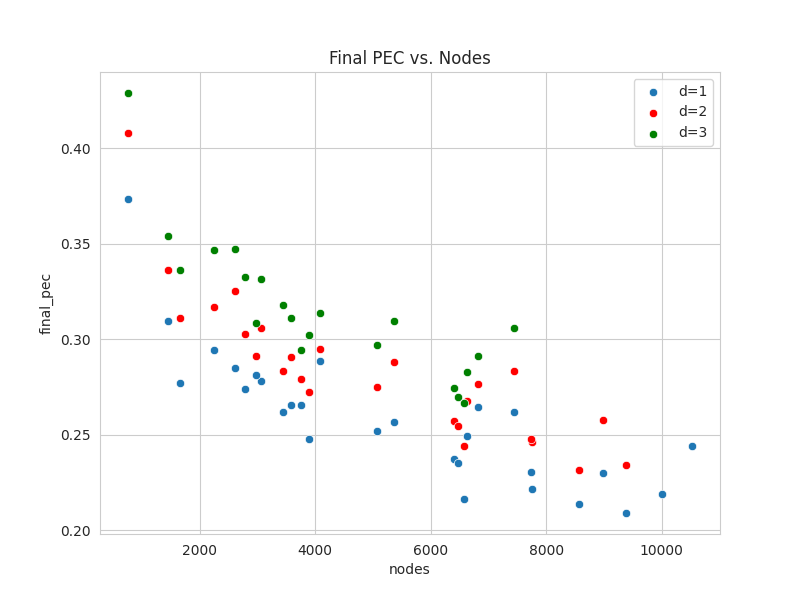
\includegraphics[width=0.9\textwidth]{figures/mcmc_ordered_final_pec.png}
  \caption{Final converged PECs for fitting 1d, 2d and 3d cube GIRGs to real-world Facebook graphs using direct ordered likelihood maximisation.
  Missing some 3d numbers as batch job exceeded allotted time.}
  \label{fig:converged_pecs}
\end{figure}


% However even when the input graph is a GIRG, we still get a similar curve (though overall higher PECs of course). One possible explanation is that we didn't reach full convergence for larger graphs - despite trying to indeed award them more iterations (and more point proposals for higher dimension).
% Not surprisingly for any given graph, $d=3 > 2 > 1$ in terms of PEC performance as having more parameters should lead to a better (potentially over-) fit.


\begin{figure}
  \centering

  \begin{subfigure}{0.49\textwidth}
    \centering
    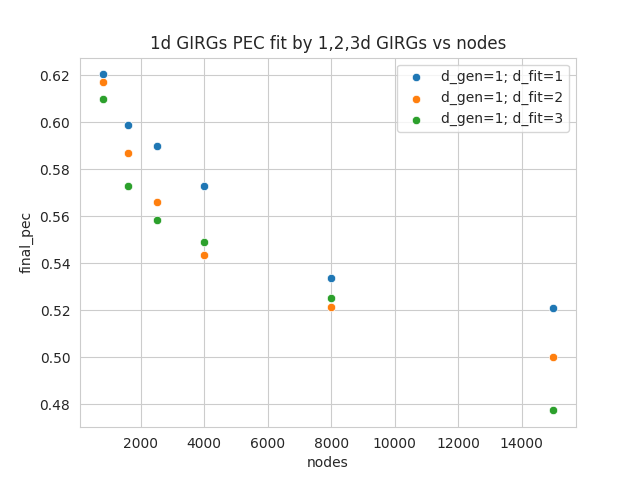
\includegraphics[width=\linewidth]{figures/mcmc_ordered_girggen_d_gen1_pecs.png}
    \caption{input graph is a 1d cube GIRG}
  \end{subfigure}
  \hfill
  \begin{subfigure}{0.49\textwidth}
    \centering
    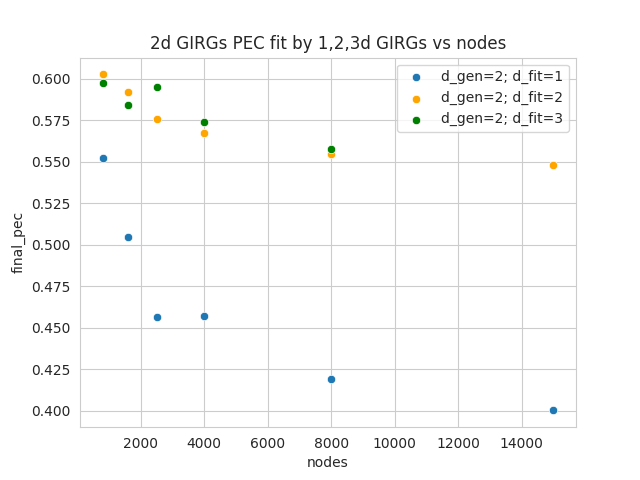
\includegraphics[width=\linewidth]{figures/mcmc_ordered_girggen_d_gen2_pecs.png}
    \caption{input graph is a 2d cube GIRG}
  \end{subfigure}

  \vspace{1em}

  \parbox[b]{.49\textwidth}{\Large
  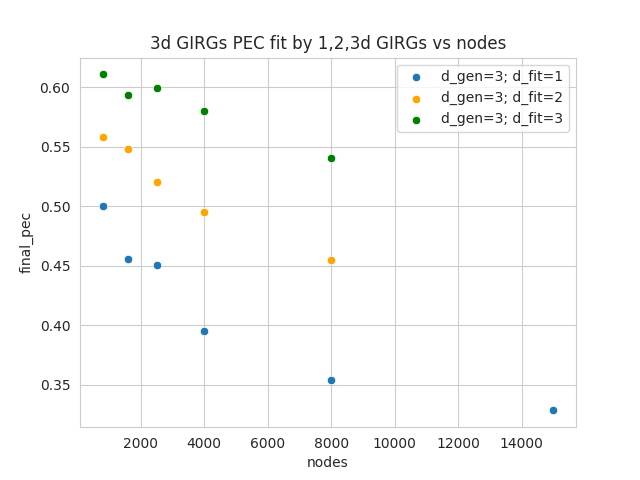
\includegraphics[width=\linewidth]{./figures/mcmc_ordered_girggen_d_gen3_pecs.png}
  \subcaption{input graph is a 3d cube GIRG}
  }
  \hfill
  \parbox[b]{.49\textwidth}{%
  \caption{Each plot shows the final PEC performance of fitting 1d, 2d and 3d cube GIRGs to an input graph of varying number of nodes. Input graphs are themselves generated from a cube GIRG - a different dimension $d=1,2,3$ for each plot.}}

  \label{fig:pec_girggen}
\end{figure}

\paragraph{Inherently low GIRG PECs}
A first thing to note is that edge probabilities $p_{uv}$ for a GIRG are generally not all $p_{uv} \in \{0, 1\}$ (at least for $\alpha < \infty$). Hence we cannot expect too high a PEC, even if we fit every single GIRG parameter perfectly to identically reproduce all the $p_{uv}$. We observe this in \cref{fig:pec_girg_identical_puv}, where PEC starts for the smallest graphs of $n=800$ nodes at $64\%$. Note the plot is of cube GIRGs generated with $\alpha=1.3$ which is quite typical an LCC fit on the real-world Facebook graphs, so indeed their edge probabilities range broadly in $[0.0, 1.0]$.

\paragraph{Fixed average degree $\implies$ lower GIRG $p_{uv}$ $\implies$ lower PECs for higher $n$}
Also striking in \cref{fig:pec_girg_identical_puv} is a similar curve to \cref{fig:converged_pecs} of decreasing PEC with increasing node count. We think this is an artifact of the fixed average degree of $\overline{deg} = 60$ used across these varying node count GIRGs. We fixed $\overline{deg}$ because the socfb graphs have basically stable average degrees - correlation coefficient of just $0.1$ with node count, and their mean average degree across graphs is $77$. We think that as $n$ grows for a fixed $\overline{deg}$, since long distance edges in a GIRG contribute a constant fraction of total edges, in order to keep average degree constant the edge probability constant $c$ is lowered. Hence for  small $n$ all edge probabilities $p_{uv}$ are generally larger and less numerous ($O(n^2)$ potential edges); for large $n$ there are many more potential edges, and generally smaller edge probabilities $p_{uv}$. This naturally brings about decreased PEC for larger $n$.

\paragraph{Fixed average degree $\implies$ lower PECs in general}
Another issue with fixed average degree and increasing $n$ is that even in the dumbest case of fitting an Erdos-Renyi graph to an input graph, we would observe a $1/n$ shaped PEC curve with increasing $n$. For each present edge in the input graph, there is a $p = \frac{\overline{deg}}{n}$ chance that it is also present in the Erdos-Renyi graph. Hence PEC would be $\frac{\overline{deg}}{n}$ in expectation.

This means that if we assume real-world graphs are only partially GIRG explainable, and that their residual non geometric random component is hence hard to fit with our low dimensional cube GIRGs, then the observed PEC against node count $n$ plot would still look like a $1/n$ curve, but with a higher non-zero asymptote.

\paragraph{Chung-Lu control shows GIRGs not overfitting on real-world}
% As a final vindication of the performance of GIRG fits to our real-world Facebook graphs, when
As a control, we fit GIRGs using direct ordered likelihood maximisation to Chung-Lu graphs, and observed PEC's is not much higher than between two resampled Chung-Lu graphs, at $10\%$ for graphs of $n=1000$ nodes, decaying to $3\%$ for $n=5000$. While there is roughly a $3\%$ PEC boost from increasing dimension $d$ which is clearly overfitting, this vindicates that the relatively higher acheived PECs of $22\% - 33\%$ in \cref{fig:converged_pecs} represent a true geometric quantity of real-graphs that we are successfully fitting.

% NB \cref{fig:pec_girggen} GIRGs were generated with $\alpha=1.3$ which is quite typical for $d=1,2,3$ cube GIRGs fit on the real-world Facebook graphs). Hence we cannot expect too high a PEC, even if we fit every single GIRG parameter perfectly to identically reproduce edge probabilities $p_{uv}$. In fact decreasing PEC with increasing node count in this case seems to be an artifact of holding the average degree constant at $\overline{deg} = 60$. If you let $\overline{deg}$ increase linearly with increasing $n$ this phenomenon seems to disappear (testing with 1d GIRGs with a range of $n=800, ..., 15000$ we get all PECs in the range $[0.62, 0.64]$). We fixed $\overline{deg}$ because the socfb graphs have basically stable average degrees - correlation coefficient of just $0.1$ with node count, and their mean average degree across graphs is $77$. I think that essentially as $n$ grows, since long distance edges contribute a constant factor of total edges, to keep average degree constant we must lower the constant $c$. Hence the comparison is small $n$, fewer larger edge probabilities vs large $n$, more, smaller edge probabilities - naturally the latter case has decreased PEC.

% TODO add results of chunglu gen girg fit as a comparison point.

Overall we find that cube GIRGs get quite a decent fit on the real-world facebook graphs, and that again 1 dimension seems already to bring a high amount of accuracy - increasing $d$ only brings small gains, e.g. looking at graphs of size about $n=8000$ nodes, the PEC increase from 1d to 2d cube GIRG fitting is just $22\% \to 25\%$. In contrast for fitting a 2d cube GIRG with a 1d cube GIRG, PEC jumps from $42\% \to 55\%$; fitting 3d with 1d PEC jumps from $0.35 \to 0.55$. We can observe in \cref{fig:uniformifed_vs_restricted_rescaling} the final fit point locations of 2d GIRGs to a few graphs (2d because this is easiest for visualisation in a plot) - we see that points for socfb-Bowdoin47 and especially socfb-Haverford76 look like they could be pretty well approximated by 1d fit locations, whereas socfb-Rice31 has more complexity going on, and an extra dimension seems important to fully capture the graph structure.



\begin{figure}
  % \parbox[b]{.69\textwidth}{\Large
  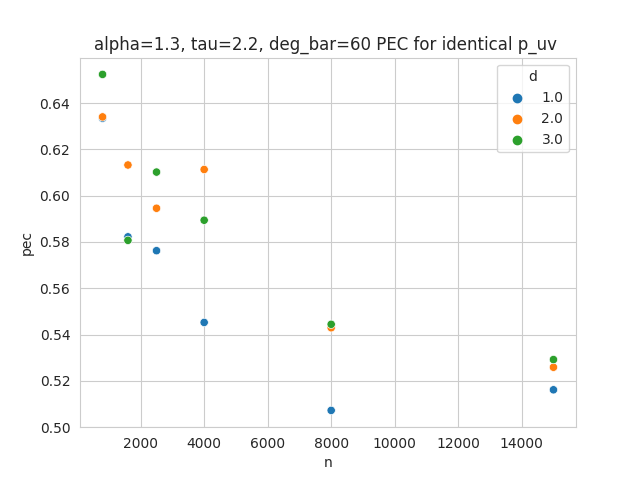
\includegraphics[width=0.8\textwidth]{./figures/pec_girg_identical_puv.png}
  % }
  \hfill
  % \parbox[b]{.3\textwidth}{%
  \caption{Exact $p_{uv}$ replication has PEC $\in [0.52, 0.64]$, and decreasing with increasing node count. Done for $\alpha=1.3, \tau=2.2$ cube GIRGs of dimension $d=1,2,3$ and average degree $60$.}
  \label{fig:pec_girg_identical_puv}
  % }
\end{figure}


% we can't directly compare $P$ to the real graph adjacency matrix $A \in \{0, 1\}^{n \times n}$. Instead we need to threshold $P$ to get a binary matrix $\hat{P} \in \{0, 1\}^{n \times n}$, and then compare $\hat{P}$ to $A$. We can do this by maximising the F1 score, which is the harmonic mean of precision and recall, and is invariant to the threshold used. We can also use the F1 score to compare two different GIRG fits to the same real graph, e.g. 1d vs 2d cube GIRG.


% TODO add in GIRG generated graphs final PEC vs Nodes plot.

% Note on the PEC plot: A simple model that might explain what's going on. Say that in the real graph it's 50\% GIRG like and 50\% random shit. So edge probabilities look like $0.5 p_1 + 0.5 p_2$, or roughly half edges are from $p_1$ (GIRG) and half edges are from $p_2$ (random). We fit a GIRG via $\hat{p}$ to observed edges. We're actually aiming at capturing 100\% of the edges, so our we have more prob mass than $0.5 p_1$, however let's say that $\hat{p}_1 = p_1 + \Delta p$. Then we fit roughly $0.5 * 0.8$ of GIRG edges and $\bar{d}/2n$ of the remaining edges. So e.g. $y = 0.5*0.8 + 0.5*60/x$. This is the simple model where GIRG edges are either $p_1 = 0$ or $p_1 = 0.8$.
% The results of running the MCMC process is to achieve PEC of about??

% TODO rerun MCMC for larger graphs for longer. We didn't seem to be converging. I.e. it seems like we need a greater than linear iteration scaling to converge??

% \begin{tabular}{|l|c|c|r|}
%   \hline
%   real graph & PEC & PEC CL & Number iterations run \\
%   \hline
%   socfb-Caltech36-1d.pkl & 0.218726 & 0.057174 & 134400 \\
%   socfb-Reed98-1d.pkl & 0.172603 & 0.039337 & 173600 \\
%   socfb-Haverford76-1d.pkl & 0.210710 & 0.058752 & 257600 \\
%   socfb-Simmons81-1d.pkl & 0.168839 & 0.030439 & 268800 \\
%   socfb-Swarthmore42-1d.pkl & 0.181657 & 0.044276 & 296800 \\
%   socfb-Amherst41-1d.pkl & 0.181718 & 0.033742 & 403200 \\
%   socfb-Bowdoin47-1d.pkl & 0.132771 & 0.033619 & 403200 \\
%   socfb-Hamilton46-1d.pkl & 0.147926 & 0.036735 & 414400 \\
%   socfb-Trinity100-1d.pkl & 0.140800 & 0.033099 & 470400 \\
%   socfb-USFCA72-1d.pkl & 0.120164 & 0.017381 & 481600 \\
%   socfb-Williams40-1d.pkl & 0.127645 & 0.029190 & 498400 \\
%   socfb-Oberlin44-1d.pkl & 0.112043 & 0.020820 & 526400 \\
%   socfb-Smith60-1d.pkl & 0.088302 & 0.021486 & 532000 \\
%   \hline
% \end{tabular}


\begin{figure}
  \centering
  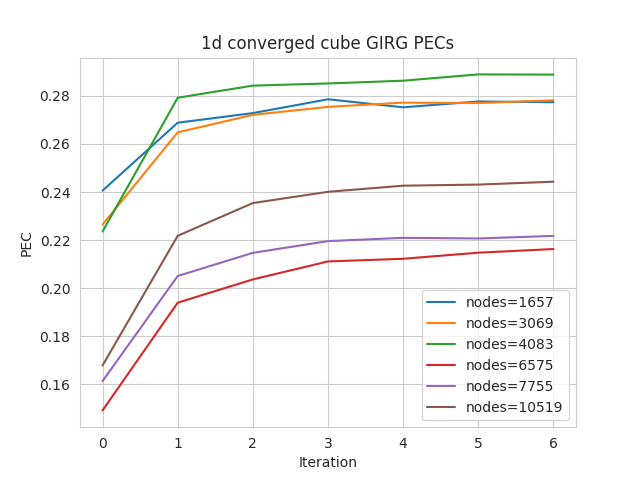
\includegraphics[width=0.49\textwidth]{figures/mcmc_ordered_1d_pec_convergence.png}
  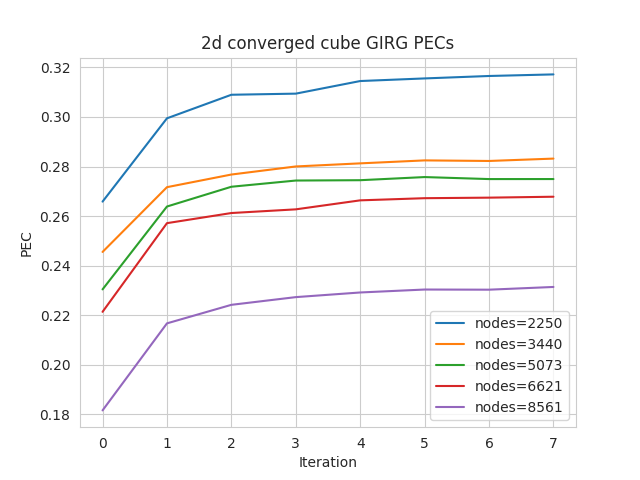
\includegraphics[width=0.49\textwidth]{figures/mcmc_ordered_2d_pec_convergence.png}
  \caption{Direct ordered likelihood maximisation PEC convergence over iterations for a range of example socfb graphs with different number of nodes. Each curve is a single fit graph. X-axis is round number, where each round every node is moved once to a new location. Y-axis is PEC after that round. We claim convergence due to plateaued PEC, and note that in general the final achieved PEC decreases with graph node count.}
  \label{fig:direct_ordered_pec_convergence_curves}
\end{figure}



% TODO further improvements might be: updating weight estimates (adding into ordered MCMC, as per mercator). Making code run on GPU.


\begin{figure}
  \caption{2d cube GIRG fitting examples, to three different Facebook graphs. Two initial 2d diffusion map embeddings are shown with either $\uniformify$ post-processing or restricted-rescaling. The blue lines for the restricted version show the border at which points are outer uniformified. Bottom two plots are heat map and scatter plots for the nodes having undergone further point location refinement using direct ordered likelihood maximisation. Note for example for socfb-Haverford76, restricted-rescaling separated the points into two (maybe even more) linear clusters which is a better initialisation, whereas $\uniformify$ was incapable of this and just produced one contiguous line of points. This also occurs to some degree for the other two graphs.}
  \label{fig:uniformifed_vs_restricted_rescaling}
  \centering

  \begin{subfigure}{\textwidth}
    \centering
    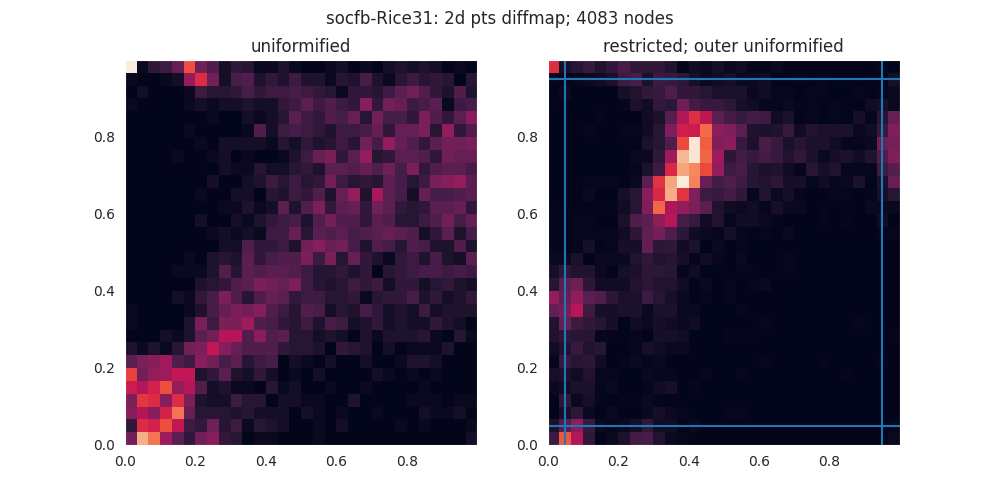
\includegraphics[width=\linewidth]{figures/socfb-Rice31_2ddiffmap_unif_vs_restrict.png}
    % \label{fig:sub1}
  \end{subfigure}

  \vspace{1em}
  \begin{subfigure}{\textwidth}
    \centering
    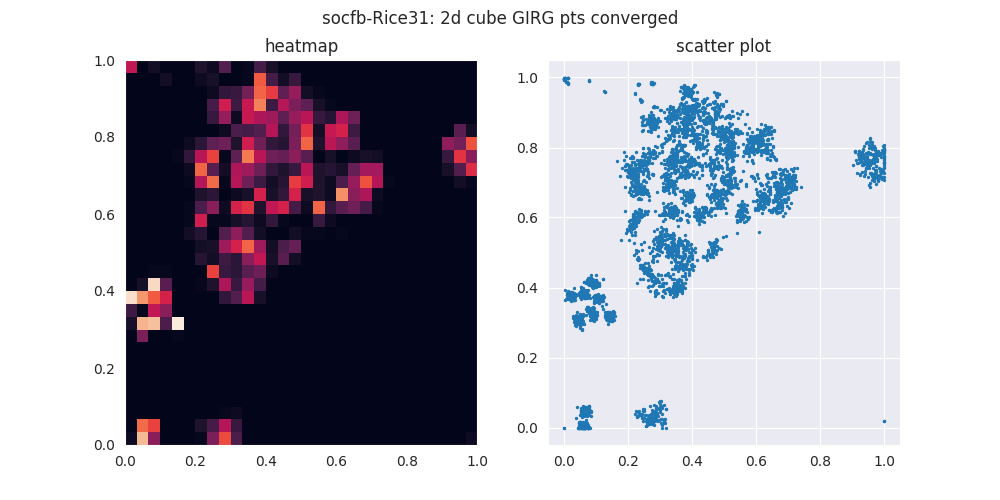
\includegraphics[width=\linewidth]{figures/socfb-Rice31_2d_cube_GIRG_converged.png}
    % \label{fig:sub1}
  \end{subfigure}

  \vspace{1em}
  
\end{figure}
\begin{figure}
  \begin{subfigure}{\textwidth}
    \centering
    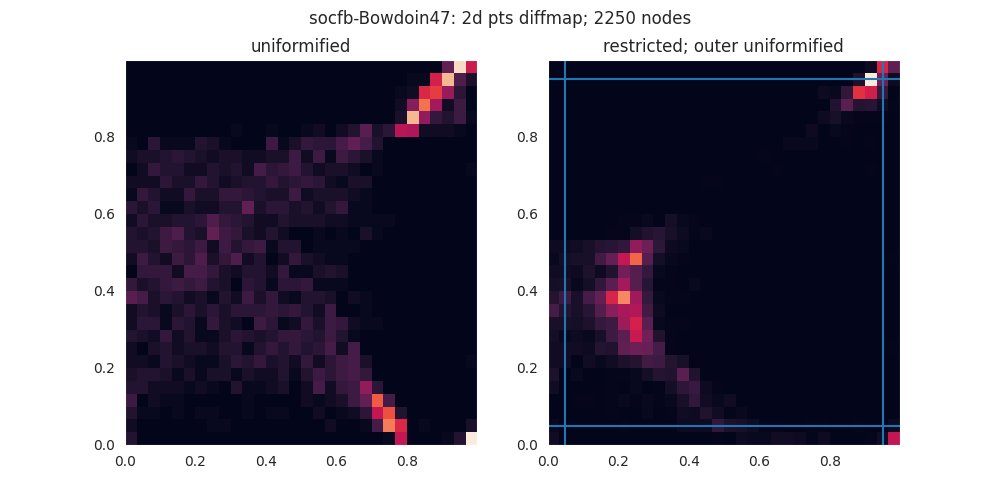
\includegraphics[width=\linewidth]{figures/socfb-Bowdoin47_2ddiffmap_unif_vs_restrict.png}
    % \label{fig:sub1}
  \end{subfigure}

  \vspace{1em}
  \begin{subfigure}{\textwidth}
    \centering
    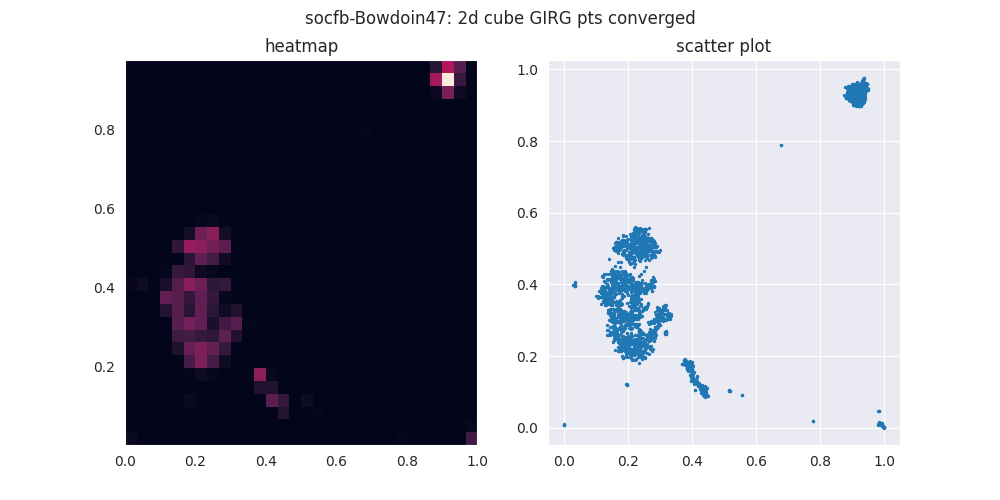
\includegraphics[width=\linewidth]{figures/socfb-Bowdoin47_2d_cube_GIRG_converged.png}
    % \label{fig:sub1}
  \end{subfigure}

\end{figure}

\begin{figure}
  \begin{subfigure}{\textwidth}
    \centering
    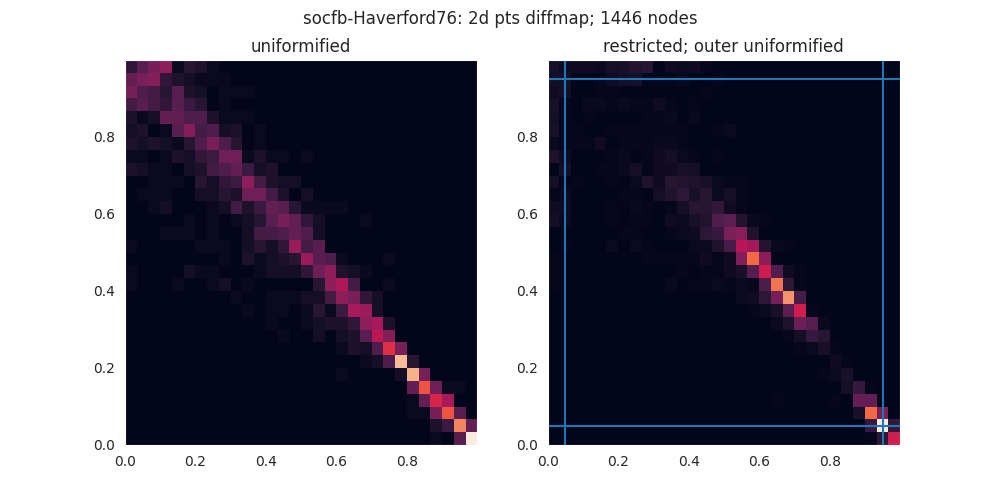
\includegraphics[width=\linewidth]{figures/socfb-Haverford76_2ddiffmap_unif_vs_restrict.png}
    % \label{fig:sub1}
  \end{subfigure}

  \vspace{1em}
  \begin{subfigure}{\textwidth}
    \centering
    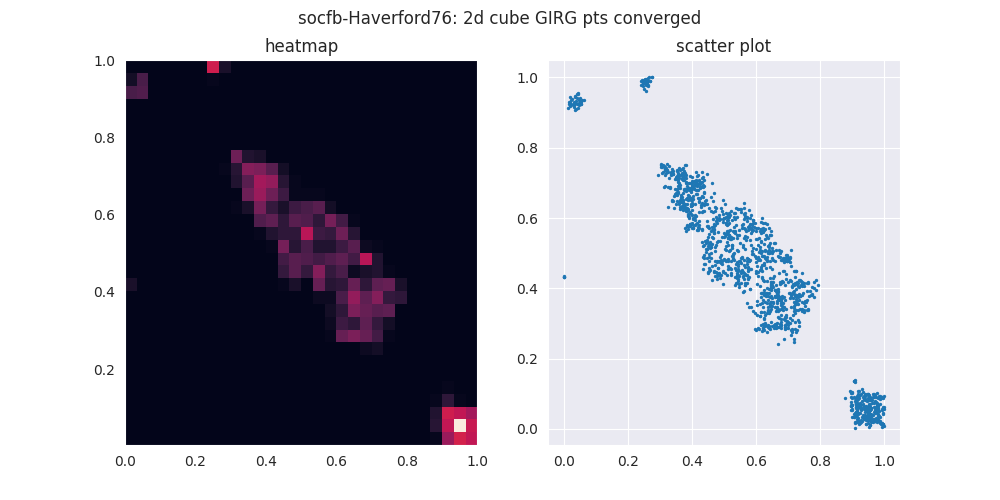
\includegraphics[width=\linewidth]{figures/socfb-Haverford76_2d_cube_GIRG_converged.png}
    % \label{fig:sub1}
  \end{subfigure}

\end{figure}


% \subsection{point initalisation and failure rate}
% Initially I ran MCMC using uniformified diffusion map initialisation, and failure rate $0.0$. The MCMC would converge, but actually take longer than necessary, as the "good" initialisation was being undone in favour of quite spaced out points.

% The evidence for this is shown in some plots of points over time:

% \begin{figure}
%   \centering
%   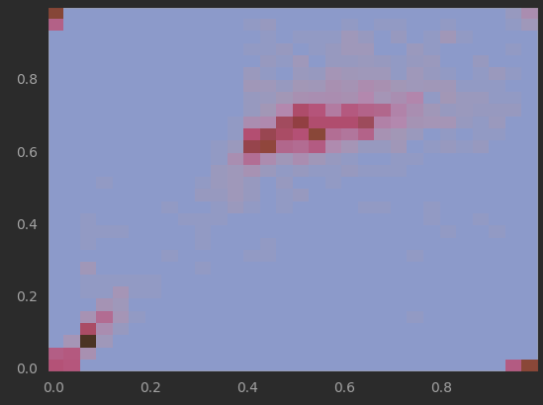
\includegraphics[width=\textwidth]{figures/amherst_2d_pts_restricted.png}
%   \caption{0.05 quantile restricted and uniformed at the edges diffusion map initialisation of MCMC points for socfb-Amherst41}
% \end{figure}

% \begin{figure}

%   \begin{subfigure}{1.0\textwidth}
%   \centering
%   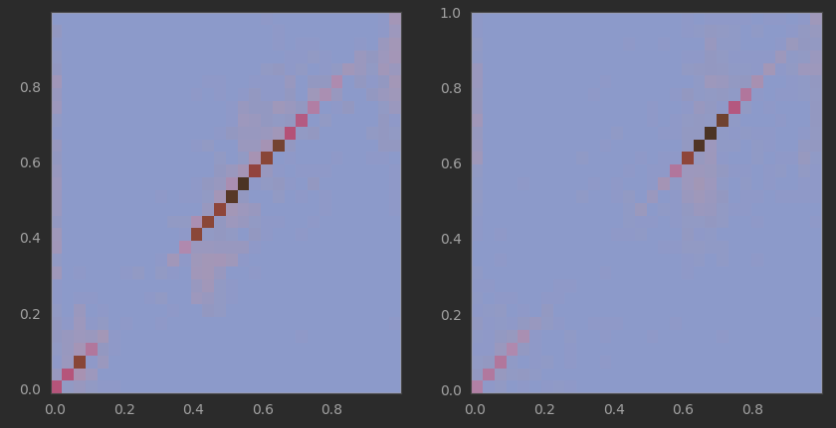
\includegraphics[width=\linewidth]{figures/amherst_failure_mcmc_pts.png}
%   \caption{failure rate $0.3$}
% \end{subfigure}

%   \vspace{1em}

%   \begin{subfigure}{1.0\textwidth}
%   \centering
%   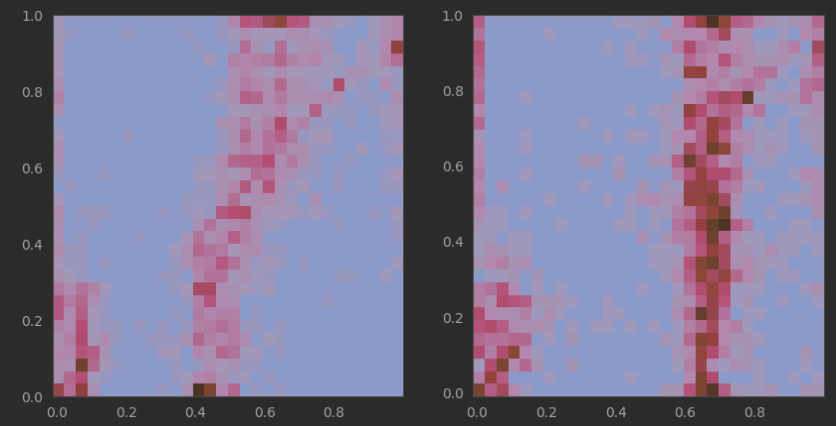
\includegraphics[width=\linewidth]{figures/amherst_nonfailure_mcmc_pts.png}
%   \caption{failure rate $0.0$ (aka no failure rate)}
% \end{subfigure}

%   \caption{MCMC iterated points scatter plot against initialisation, with/without failure rate}
%   \label{fig:amherst_points_over_time}
% \end{figure}


% Run long enough, the MCMC's points converge to the cube:

% \begin{figure}
%   \centering
%   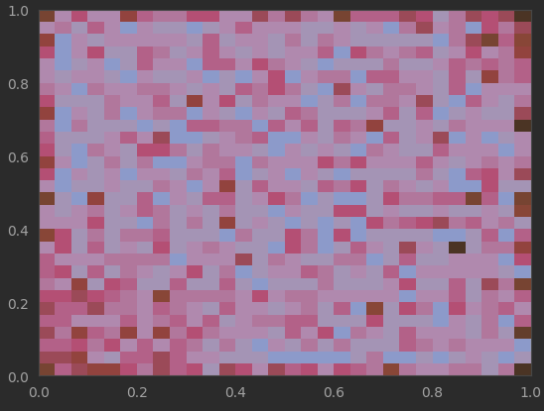
\includegraphics[width=\textwidth]{figures/MCMC_converged_to_cube.png}
%   \caption{failure rate $0.0$ run until convergence for 2D GIRG: points 2D histogram}
% \end{figure}


% \begin{table}[ht]
%   \centering
%   \begin{tabular}{|l|l|}
%   \hline
%   \textbf{LL maximum for 1D} & \textbf{LL maximum for 2D} \\
%   \hline
%   socfb-Amherst41 & socfb-Bowdoin47 \\
%   socfb-Oberlin44 & socfb-Caltech36 \\
%   socfb-Reed98 & socfb-Colgate88 \\
%   socfb-Swarthmore42 & socfb-Hamilton46 \\
%   socfb-Wellesley22 & socfb-Haverford76 \\
%   & socfb-Middlebury45 \\
%   & socfb-Pepperdine86 \\
%   & socfb-Santa74 \\
%   & socfb-Simmons81 \\
%   & socfb-Smith60 \\
%   & socfb-Trinity100 \\
%   & socfb-USFCA72 \\
%   & socfb-Vassar85 \\
%   & socfb-Williams40 \\
%   \hline
%   \end{tabular}
%   \caption{Your Caption}
%   \label{tab:my_label}
%   \end{table}




